\documentclass[a4paper,12pt]{exam}
\usepackage{graphicx}
\usepackage[document]{ragged2e}
 \usepackage[margin=1in]{geometry}
\usepackage{circuitikz}
\usepackage{tikz}
\usetikzlibrary{arrows.meta, shapes, circuits.ee.IEC, positioning}
\usepackage{float}
\usepackage{amsmath}
\usepackage{multicol}
\usepackage{enumitem}
\usepackage{setspace}
\usepackage{amssymb}

\usepackage{cite}
\usepackage{graphicx}
\usepackage{amsmath,amssymb,amsfonts,amsthm}
\usepackage{algorithmic}
\usepackage{graphicx}
\usepackage{textcomp}
\usepackage{xcolor}
\usepackage{txfonts}
\usepackage{listings}
\usepackage{enumitem}
\usepackage{mathtools}
\usepackage{gensymb}
\usepackage{comment}
\usepackage[breaklinks=true]{hyperref}
\usepackage{tkz-euclide} 
\usepackage{listings}
\usepackage{gvv}                                        
%\def\inputGnumericTable{}                                 
\usetikzlibrary{arrows.meta, positioning}
\usepackage{xparse}
\usepackage{color}                                            
\usepackage{array}                                            
\usepackage{longtable}                                       
\usepackage{calc}                                             
\usepackage{multirow}
\usepackage{multicol}
\usepackage{hhline}                                           
\usepackage{ifthen}                                           
\usepackage{lscape}
\usepackage{tabularx}
\usepackage{array}
\usepackage{float}
\newtheorem{theorem}{Theorem}[section]
\newtheorem{problem}{Problem}
\newtheorem{proposition}{Proposition}[section]
\newtheorem{lemma}{Lemma}[section]
\newtheorem{corollary}[theorem]{Corollary}
\newtheorem{example}{Example}[section]
\newtheorem{definition}[problem]{Definition}
\newcommand{\BEQA}{\begin{eqnarray}}
\newcommand{\EEQA}{\end{eqnarray}}
\usepackage{float}
%\newcommand{\define}{\stackrel{\triangle}{=}}
\theoremstyle{remark}
\usepackage{circuitikz}
\usepackage{tikz}
\usepackage{ragged2e}


\begin{document}
\begin{figure}[H]
    \centering
    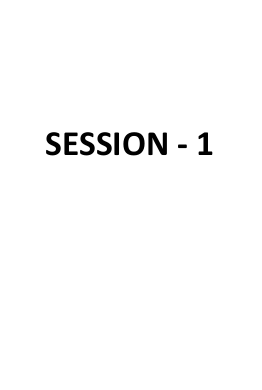
\includegraphics[width=1\columnwidth]{figs/image1.png}
\end{figure}
\newpage
  \begin{center}
\textbf{ Graduate Aptitude Test in Engineering}
  \end{center}
\textbf{Question Paper Name:}\quad EE:ELECTRICAL ENGINEERING 7th Feb Shift 1\\
\textbf{Number of Questions   :}\quad 65\\
\textbf{Total Marks:}\qquad \qquad \quad 100.0\\
\vspace{0.5cm}
Wrong answer for MCQ will result in negative marks, (-1/3) for 1 mark Questions and (-2/3) for 2 marks \\
\vspace{0.5cm}
General Aptitude\\
Number of Questions: 10\\
Section Marks: 15.0\\
\vspace{0.5cm}
 Q.1 to Q.5 carry 1 mark each \& Q.6 to Q.10 carry 2 marks
\begin{enumerate}
\item Didn't you buy \rule{3cm}{0.15mm} when you went shopping?\hfill{\textbf{(GATE EE 2015)}} 
    \begin{multicols}{4}
    \begin{enumerate}   
        \item any paper
        \item much paper
        \item no paper
        \item a few paper
    \end{enumerate}
    \end{multicols}

\item Which of the following options is the closest in meaning to the sentence below?\\
She enjoyed herself immensely at the party.\hfill{\textbf{(GATE EE 2015)}}
   
    \begin{enumerate}   
        \item She had a terrible time at the party
        \item She had a horrible time at the party
        \item She had a terrific time at the party
        \item She had a terrifying time at the party
    \end{enumerate}
 

\item Which one of the following combinations is incorrect?\hfill{\textbf{(GATE EE 2015)}}
    \begin{multicols}{2}
    \begin{enumerate}   
        \item Acquiescence - Submission
        \item Wheedle - Roundabout
        \item Flippancy - Lightness
        \item Profligate - Extravagant
    \end{enumerate}
    \end{multicols}

\item Based on the given statements, select the most appropriate option to solve the given question.\\
If two floors in a certain building are 9 feet apart, how many steps are there in a set of stairs that extends from the first floor to the second floor of the building?\\
Statements:
\begin{enumerate} 
\item[(I)] Each step is 3/4 foot high.
\item[(II)] Each step is 1 foot wide.\hfill{\textbf{(GATE EE 2015)}}
\end{enumerate}
  
    \begin{enumerate}   
        \item Statement I alone is sufficient, but statement II alone is not sufficient.
        \item Statement II alone is sufficient, but statement I alone is not sufficient.
        \item Both statements together are sufficient, but neither statement alone is sufficient.
        \item Statement I and II together are not sufficient.
    \end{enumerate}
  \newpage

\item Given Set $A = \{2, 3, 4, 5\}$ and Set $B = \{11, 12, 13, 14, 15\}$, two numbers are randomly selected, one from each set. What is the probability that the sum of the two numbers equals 16?\hfill{\textbf{(GATE EE 2015)}}
    \begin{multicols}{4}
    \begin{enumerate}   
        \item 0.20
        \item 0.25
        \item 0.30
        \item 0.33
    \end{enumerate}
    \end{multicols}
\item Select the alternative meaning of the underlined part of the sentence.\\
The chain snatchers \underline{took to their heels} when the police party arrived.\hfill{\textbf{(GATE EE 2015)}}
    \begin{multicols}{4}
    \begin{enumerate}
        \item took shelter in a thick jungle
        \item open indiscriminate fire
        \item took to flight
        \item unconditionally surrendered
    \end{enumerate}
    \end{multicols}

\item The given statement is followed by some courses of action. Assuming the statement to be true, decide the correct option.\hfill{\textbf{(GATE EE 2015)}}\\
Statement:\\
There has been a significant drop in the water level in the lakes supplying water to the city.\\
Course of action:\\
\begin{enumerate}
\item[(I)] The water supply authority should impose a partial cut in supply to tackle the situation.
\item[(II)] The government should appeal to all the residents through mass media for minimal use of water.
\item[(III)] The government should ban the water supply in lower areas.
\end{enumerate}
    \begin{multicols}{2}
    \begin{enumerate}   
        \item Statements I and II follow.
        \item Statements I and III follow.
        \item Statements II and III follow.
        \item All statements follow.
    \end{enumerate}
    \end{multicols}
\item The pie chart below has the breakup of the number of students from different departments in anengineering college for the year 2012. The proportion of male to female students in each
department is 5:4. There are 40 males in Electrical Engineering. What is the difference between the numbers of female students in the Civil department and the female students in the Mechanical department?\hfill{\textbf{(GATE EE 2015)}}
\begin{figure}[H]
    \centering
    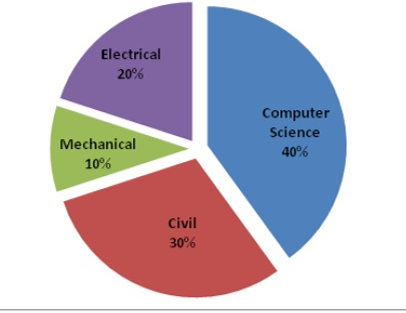
\includegraphics[width=0.5\columnwidth]{figs/Q 8.png}
    \caption{}
    \label{fig:placeholder}
\end{figure}
\newpage
\item The probabilities that a student passes in Mathematics, Physics and Chemistry are m, p, and c respectively. Of these subjects, the student has 75\% chance of passing in at least one, a 50\% chance of passing in at least two and a 40\% chance of passing in exactly two. Following relations are drawn in m, p, c:\\
(I) p + m + c = 27/20\\
(II) p + m + c = 13/20\\
(III) (p) × (m) × (c) = 1/10\hfill{\textbf{(GATE EE 2015)}}\\

\begin{enumerate}
  \item Only relation I is true.
  \item Only relation II is true.
  \item Relations II and III are true.
  \item Relations I and III are true.
\end{enumerate}

\item The number of students in a class who have answered correctly, wrongly, or not attempted each question in an exam, are listed in the table below. The marks for each question are also listed. There is no negative or partial marking.\hfill{\textbf{(GATE EE 2015)}}

\begin{tabular}{|c|c|c|c|c|}
\hline
Q No. & Marks & Answered Correctly & Answered Wrongly & Not Attempted \\
\hline
1 & 2 & 21 & 17 & 6 \\
2 & 3 & 15 & 27 & 2 \\
3 & 1 & 11 & 29 & 4 \\
4 & 2 & 23 & 18 & 3 \\
5 & 5 & 31 & 12 & 1 \\
\hline
\end{tabular}

What is the average of the marks obtained by the class in the examination?
\begin{multicols}{4}
\begin{enumerate}
  \item 2.290
  \item 2.970
  \item 6.795
  \item 8.795
\end{enumerate}
\end{multicols}
\centering{ELECTRICAL ENGINNEERING}\\
Number of Questions:55\\
 Section Marks: 85\\
 \vspace{0.5cm
 }
\raggedright{ Q.11 to Q.35 carry 1 mark each \& Q.36 to Q.65 carry 2 marks each.}
\item A random variable    $X   $ has probability density function\hfill{\textbf{(GATE EE 2015)}}\\ $ f(x) = \begin{cases} a + bx, & 0 < x < 1 \\ 0, & \text{otherwise} \end{cases} $.

If the expected value $E[X] = \frac{2}{3}$, then $\Pr[X < 0.5]$ is \rule{3cm}{0.15mm}.

\item If a continuous function f(x) does not have a root in the interval $[a,b]$, then which one of the following statements is TRUE?\hfill{\textbf{(GATE EE 2015)}}

\begin{enumerate}
  \item    $f(a) \cdot f(b) = 0   $
  \item    $f(a) \cdot f(b) < 0   $
  \item    $f(a) \cdot f(b) > 0   $
  \item    $\frac{f(a)}{f(b)} \leq 0   $
\end{enumerate}

\item If the sum of the diagonal elements of a    $2 \times 2   $ matrix is -6, then the maximum possible value of the determinant of the matrix is \rule{3cm}{0.15mm}.\hfill{\textbf{(GATE EE 2015)}}

\item Consider a function    $\mathbf{f} = \frac{\hat{r}}{r^2}   $, where    $r   $ is the distance from the origin and    $\hat{r}   $ is the unit vector in the radial direction. The divergence of this function over a sphere of radius R, which includes the origin, is\hfill{\textbf{(GATE EE 2015)}}
\begin{multicols}{4}
\begin{enumerate}
  \item 0
  \item    $2\pi   $
  \item    $4\pi   $
  \item    $R \pi   $
\end{enumerate}
\end{multicols}
\item When the Wheatstone bridge shown in the figure is used to find the value of resistor    $R_x   $, the galvanometer    $G   $ indicates zero current when    $R_1 = 50 \Omega   $,    $R_2 = 65 \Omega   $, and    $R_3 = 100 \Omega   $. If    $R_3   $ is known with    $\pm 5\%   $ tolerance on its nominal value of 100    $\Omega   $, what is the range of    $R_x   $ in Ohms? \hfill{\textbf{(GATE EE 2015)}}
\begin{figure}[H]
    \centering
    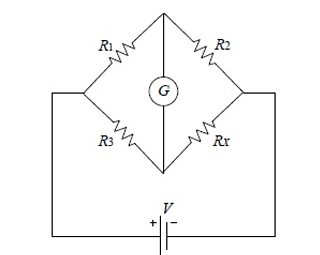
\includegraphics[width=0.5\columnwidth]{figs/Q 15.png}
    \caption{}
    \label{fig:placeholder}
\end{figure}
\begin{multicols}{2}
\begin{enumerate}
    \item $[a]$    $[123.50, 136.50]   $
    \item [B]    $[125.89, 134.12]   $
    \item [C]    $[117.00, 143.00]   $
    \item [D]    $[120.25, 139.75]   $
\end{enumerate}
\end{multicols}
\item A    $(0-50 \text{ A})   $ moving coil ammeter has a voltage drop of 0.1 V across its terminals at full scale deflection. The external shunt resistance (in milliohms) needed to extend its range to    $(0-500 \text{ A})   $ is \rule{3cm}{0.15mm}.\hfill{\textbf{(GATE EE 2015)}}

\item Of the four characteristics given below, which are the major requirements for an instrumentation amplifier?\hfill{\textbf{(GATE EE 2015)}}
\begin{enumerate}
    \item P. High common mode rejection ratio
    \item Q. High input impedance
    \item R. High linearity
    \item S. High output impedance
\end{enumerate}
\begin{multicols}{2}
\begin{enumerate}
    \item P, Q, and R only
    \item P and R only
    \item P, Q, and S only
    \item Q, R, and S only
\end{enumerate}
\end{multicols}

\item In the following chopper, the duty ratio of switch    $S   $ is 0.4. If the inductor and capacitor are sufficiently large to ensure continuous inductor current and ripple free capacitor voltage, the charging current (in Ampere) of the 5 V battery, under steady-state, is \rule{3cm}{0.15mm}.\hfill{\textbf{(GATE EE 2015)}}
\begin{figure}[h]
    \centering
    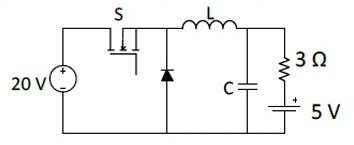
\includegraphics[width=0.5\columnwidth]{figs/Q 18.png}
    \caption{}
    \label{fig:placeholder}
\end{figure}
\item A moving average function is given by    $ y(t) =
\frac{1}{T} \int_{t-T}^{t} u(\tau)\, d\tau.
    $. If the input    $u   $ is a sinusoidal signal of frequency Hz, then in steady state, the output    $y   $ will lag    $u   $ (in degree) by \rule{3cm}{0.15mm}.\hfill{\textbf{(GATE EE 2015)}}

\item The impulse response    $g(t)   $ of a system,    $G   $, is as shown in Figure (a). What is the maximum value attained by the impulse response of two cascaded blocks of    $G   $ as shown in Figure (b)?\hfill{\textbf{(GATE EE 2015)}}
\begin{figure}[H]
    \centering
    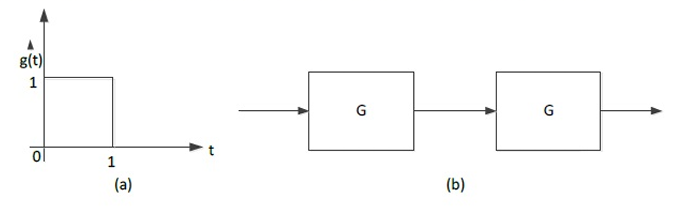
\includegraphics[width=0.5\columnwidth]{figs/Q 20.png}
    \caption{}
    \label{fig:placeholder}
\end{figure}
\begin{multicols}{4}
\begin{enumerate}
    \item    $\frac{2}{3}   $
    \item    $\frac{3}{4}   $
    \item    $\frac{4}{5}   $
    \item 1
\end{enumerate}
\end{multicols}
\item Consider a one-turn rectangular loop of wire placed in a uniform magnetic field as shown in the figure. The plane of the loop is perpendicular to the field lines. The resistance of the loop is $0.4\,\Omega$, and its inductance is negligible. The magnetic flux density (in Tesla) is a function of time, and is given by $B(t) = 0.25\sin \omega t$, where $\omega = 2\pi \times 50$ radian/second. The power absorbed (in Watt) by the loop from the magnetic field is \rule{3cm}{0.15mm}.\hfill{\textbf{(GATE EE 2015)}}
\begin{figure}[H]
    \centering
    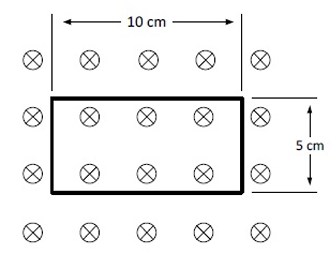
\includegraphics[width=0.4\columnwidth]{figs/Q 21.png}
    \caption{}
    \label{fig:placeholder}
\end{figure}
\newpage
\item A steady current $I$ is flowing in the $-x$ direction through each of two infinitely long wires at $y = \pm \frac{L}{2}$ as shown in the figure. The permeability of the medium is $\mu_0$. The $\vec{B}$-field at $(0, L, 0)$ is\hfill{\textbf{(GATE EE 2015)}}
\begin{figure}[H]
    \centering
    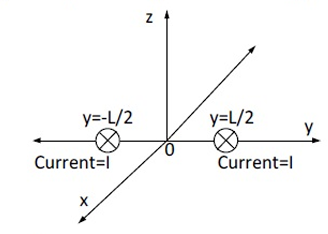
\includegraphics[width=0.5\columnwidth]{figs/Q 22.png}
    \caption{}
    \label{fig:placeholder}
\end{figure}
\begin{multicols}{4}
    \begin{enumerate}
        \item $-\dfrac{4 \mu_0 I}{3 \pi L} \, \hat{z}$
        \item $+\dfrac{4 \mu_0 I}{3 \pi L} \, \hat{z}$
        \item $0$
        \item $-\dfrac{3 \mu_0 I}{4 \pi L} \, \hat{z}$
    \end{enumerate}
\end{multicols}
\item Consider the circuit shown in the figure. In this circuit $R = 1\,\mathrm{k}\Omega$, and $C = 1\,\mu\mathrm{F}$. The input voltage is sinusoidal with a frequency of 50 Hz, represented as a phasor with magnitude $V_i$ and phase angle 0 radian as shown in the figure. The output voltage is represented as a phasor with magnitude $V_o$ and phase angle $\delta$ radian. What is the value of the output phase angle $\delta$ (in radian) relative to the phase angle of the input voltage?\\\hfill{\textbf{(GATE EE 2015)}}
\begin{figure}[H]
    \centering
    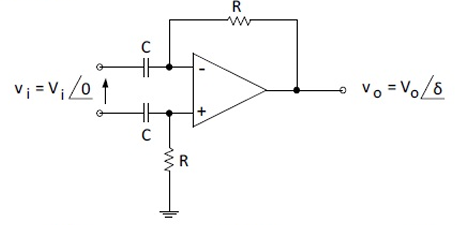
\includegraphics[width=0.5\columnwidth]{figs/Q 23.png}
    \caption{}
    \label{fig:placeholder}
\end{figure}
\begin{multicols}{4}
    \begin{enumerate}
        \item $0$
        \item $\pi$
        \item $\pi/2$
        \item $-\pi/2$
    \end{enumerate}
\end{multicols}
\item In the given circuit, the silicon transistor has $\beta = 75$ and a collector voltage $V_C = 9\,\mathrm{V}$. Then the ratio of $R_B$ and $R_C$ is \rule{3cm}{0.15mm}.\hfill{\textbf{(GATE EE 2015)}}
\begin{figure}[H]
    \centering
    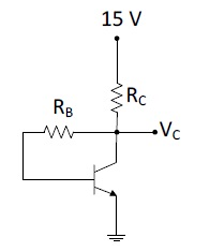
\includegraphics[width=0.4\columnwidth]{figs/Q 24.png}
    \caption{}
    \label{fig:placeholder}
\end{figure}
\item In the $4 \times 1$ multiplexer, the output $F$ is given by $F = A \oplus B$. Find the required input $I_3I_2I_1I_0$.\hfill{\textbf{(GATE EE 2015)}}
\begin{figure}[H]
    \centering
    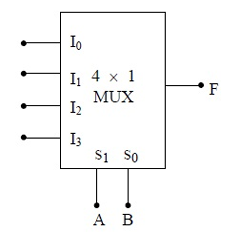
\includegraphics[width=0.5\columnwidth]{figs/Q 25.png}
    \caption{}
    \label{fig:placeholder}
\end{figure}
\begin{multicols}{4}
    \begin{enumerate}
        \item 1010
        \item 0110
        \item 1000
        \item 1110
    \end{enumerate}
\end{multicols}
\item Consider a HVDC link which uses thyristor based line-commutated converters as shown in the figure. For a power flow of 750 MW from System 1 to System 2, the voltages at the two ends, and the current, are given by: $V_1 = 500$ kV, $V_2 = 485$ kV and $I = 1.5$ kA. If the direction of power flow is to be reversed (that is, from System 2 to System 1) without changing the electrical connections, then which one of the following combinations is feasible?\hfill{\textbf{(GATE EE 2015)}}
\begin{figure}[H]
    \centering
    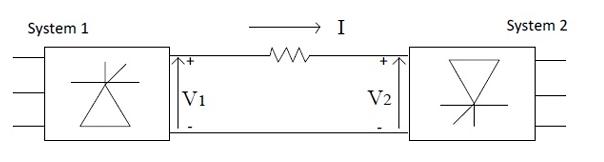
\includegraphics[width=0.5\columnwidth]{figs/Q 26.png}
    \caption{}
    \label{fig:placeholder}
\end{figure}
    \begin{enumerate}
        \item $V_1 = -500$ kV, $V_2 = -485$ kV and $I = 1.5$ kA
        \item $V_1 = -485$ kV, $V_2 = -500$ kV and $I = 1.5$ kA
        \item $V_1 = 500$ kV, $V_2 = 485$ kV and $I = -1.5$ kA
        \item $V_1 = -500$ kV, $V_2 = -485$ kV and $I = -1.5$ kA
    \end{enumerate}

\item Base load power plants are\hfill{\textbf{(GATE EE 2015)}}\\
P: wind farms.\\
Q: run-of-river plants.\\
R: nuclear power plants.\\
S: diesel power plants.
\begin{multicols}{2}
    \begin{enumerate}
        \item P, Q and S only
        \item P, R and S only
        \item P, Q and R only
        \item Q and R only
    \end{enumerate}
\end{multicols}
\item The voltages developed across the $3\,\Omega$ and $2\,\Omega$ resistors shown in the figure are 6 V and 2 V respectively, with the polarity as marked. What is the power (in Watt) delivered by the 5 V voltage source?\hfill{\textbf{(GATE EE 2015)}}
\begin{figure}[H]
    \centering
    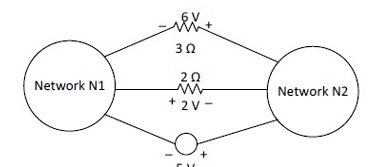
\includegraphics[width=0.5\columnwidth]{figs/Q 28.png}
    \caption{}
    \label{fig:placeholder}
\end{figure}
\begin{multicols}{4}
    \begin{enumerate}
        \item 5
        \item 7
        \item 10
        \item 14
    \end{enumerate}
\end{multicols}
\item For the given circuit, the Thevenin equivalent is to be determined. The Thevenin voltage, $V_{Th}$ (in Volt), seen from terminal AB is \rule{3cm}{0.15mm}.\hfill{\textbf{(GATE EE 2015)}}
\begin{figure}[H]
    \centering
    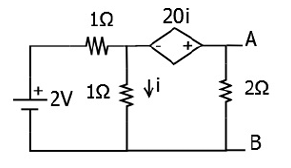
\includegraphics[width=0.4\columnwidth]{figs/Q 29.png}
    \caption{}
    \label{fig:placeholder}
\end{figure}
\item An inductor is connected in parallel with a capacitor as shown in the figure
\begin{figure}[H]
    \centering
    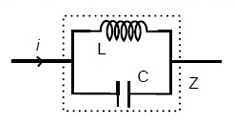
\includegraphics[width=0.5\columnwidth]{figs/Q 30.png}
    \caption{}
    \label{fig:placeholder}
\end{figure}
As the frequency of current $i$ is increased, the increased, the impedence ($Z$) of the network varies as\hfill{\textbf{(GATE EE 2015)}}
\begin{figure}[H]
    \centering
    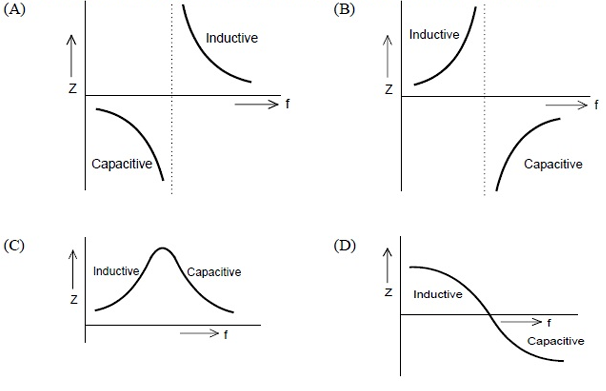
\includegraphics[width=0.9\columnwidth]{figs/Q 30 opt.png}
\end{figure}

\item A separately excited DC generator has an armature resistance of $0.1\,\Omega$ and negligible armature inductance. At rated field current and rated rotor speed, its open-circuit voltage is $200$ V. When this generator is operated at half the rated speed, with half the rated field current, an uncharged $1000\,\mu$F capacitor is suddenly connected across the armature terminals. Assume that the speed remains unchanged during the transient. At what time (in microsecond) after the capacitor is connected will the voltage across it reach 25 V?\hfill{\textbf{(GATE EE 2015)}}
\begin{multicols}{4}
    \begin{enumerate}
        \item 62.25
        \item 69.3
        \item 73.25
        \item 77.3
    \end{enumerate}
\end{multicols}
\item The self inductance of the primary winding of a single phase, 50 Hz, transformer is $800$ mH, and that of the secondary winding is $600$ mH. The mutual inductance between these two windings is $480$ mH. The secondary winding of this transformer is short circuited and the primary winding is connected to a 50 Hz, single phase, sinusoidal voltage source. The current flowing in both the windings is less than their respective rated currents. The resistance of both windings can be neglected. In this condition, what is the effective inductance (in mH) seen by the source?\hfill{\textbf{(GATE EE 2015)}}
\begin{multicols}{4}
    \begin{enumerate}
        \item 416
        \item 440
        \item 200
        \item 920
    \end{enumerate}
\end{multicols}
\item The primary mmf is least affected by the secondary terminal conditions in a\\ \hfill{\textbf{(GATE EE 2015)}}
\begin{multicols}{2}
    \begin{enumerate}
        \item power transformer
        \item potential transformer
        \item current transformer
        \item distribution transformer
    \end{enumerate}
\end{multicols}
\item A Bode magnitude plot for the transfer function $G(s)$ of a plant is shown in the figure. Which one of the following transfer functions best describes the plant?\hfill{\textbf{(GATE EE 2015)}}
\begin{figure}[H]
    \centering
    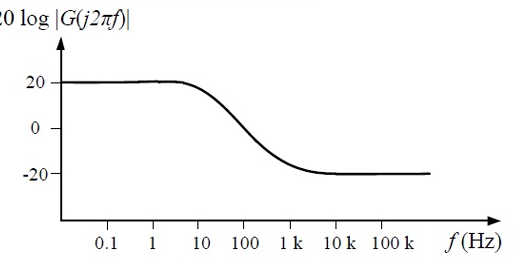
\includegraphics[width=0.5\columnwidth]{figs/Q 34.png}
    \caption{}
    \label{fig:placeholder}
\end{figure}
\begin{multicols}{4}
    \begin{enumerate}
        \item $\dfrac{1000(s+10)}{s+1000}$
        \item $\dfrac{10(s+10)}{s(s+1000)}$
        \item $\dfrac{s+1000}{10s(s+10)}$
        \item $\dfrac{s+1000}{10(s+10)}$
    \end{enumerate}
\end{multicols}
\item For the signal-flow graph shown in the figure, which one of the following expressions is equal to the transfer function $\dfrac{Y(s)}{X_2(s)|_{X_1(s)=0}}$?\hfill{\textbf{(GATE EE 2015)}}
\begin{figure}[H]
    \centering
    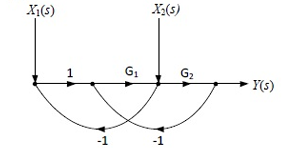
\includegraphics[width=0.5\columnwidth]{figs/Q 35.png}
    \caption{}
    \label{fig:placeholder}
\end{figure}
\begin{multicols}{4}
    \begin{enumerate}
        \item $\dfrac{G_1}{1 + G_2(1 + G_1)}$
        \item $\dfrac{G_2}{1 + G_1(1 + G_2)}$
        \item $\dfrac{G_1}{1 + G_1G_2}$
        \item $\dfrac{G_2}{1 + G_1G_2}$
    \end{enumerate}
\end{multicols}
\item The maximum value of $a$ such that the matrix
$
\myvec{
-3 & 0 & 0 & -2 \\
1 & -1 & 0 & 0 \\
0 & a & -2
}
$
has three linearly independent real eigenvectors is\hfill{\textbf{(GATE EE 2015)}}
\begin{multicols}{4}
    \begin{enumerate}
        \item $\dfrac{2}{3\sqrt{3}}$
        \item $\dfrac{1}{3\sqrt{3}}$
        \item $\dfrac{1+2\sqrt{3}}{3\sqrt{3}}$
        \item $\dfrac{1+\sqrt{3}}{3\sqrt{3}}$
    \end{enumerate}
\end{multicols}
\item A solution of the ordinary differential equation $\dfrac{d^2y}{dt^2} + 5\dfrac{dy}{dt} + 6y = 0$ is such that $y(0) = 2$ and $y(1) = -1 - \dfrac{3}{e^3}$. The value of $\frac{dy}{dt}(0)$ is \rule{3cm}{0.15mm}.\hfill{\textbf{(GATE EE 2015)}}
\item The signum function is given by
$
sgn(x) =
\begin{cases}
\dfrac{x}{|x|}, & x \neq 0 \\
0, & x = 0
\end{cases}
$
The Fourier series expansion of $sgn(\cos(t))$ has\hfill{\textbf{(GATE EE 2015)}}
    \begin{enumerate}
        \item only sine terms with all harmonics.
        \item only cosine terms with all harmonics.
        \item only sine terms with even numbered harmonics.
        \item only cosine terms with odd numbered harmonics.
    \end{enumerate}

\item Two players, A and B, alternately keep rolling a fair dice. The person to get a six first wins the game. Given that player A starts the game, the probability that A wins the game is\hfill{\textbf{(GATE EE 2015)}}
\begin{multicols}{4}
        \begin{enumerate}
        \item $5/11$
        \item $1/2$
        \item $7/13$
        \item $6/11$
    \end{enumerate}
\end{multicols}

\item An unbalanced DC Wheatstone bridge is shown in the figure. At what value of $p$ will the magnitude of $V_0$ be maximum?\hfill{\textbf{(GATE EE 2015)}}
\begin{figure}[H]
    \centering
    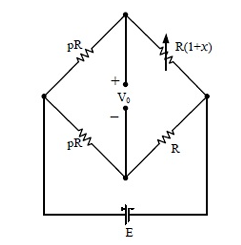
\includegraphics[width=0.4\columnwidth]{figs/Q 40.png}
    \caption{}
    \label{fig:placeholder}
\end{figure}
\begin{multicols}{4}
    \begin{enumerate}
        \item $\sqrt{1 + x}$
        \item $1 + x$
        \item $1 / \sqrt{1 + x}$
        \item $\sqrt{1 - x}$
    \end{enumerate}
\end{multicols}
\item The circuit shown is meant to supply a resistive load $R_L$ from two separate DC voltage sources. The switches S1 and S2 are controlled so that only one of them is ON at any instant. S1 is turned on for 0.2 ms and S2 is turned on for 0.3 ms in a 0.5 ms switching cycle time period. Assuming continuous conduction of the inductor current and negligible ripple on the capacitor voltage, the output voltage $V_o$ (in Volt) across $R_L$ is \rule{3cm}{0.15mm}.\hfill{\textbf{(GATE EE 2015)}}
\begin{figure}[H]
    \centering
    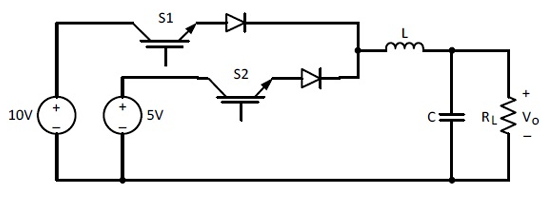
\includegraphics[width=0.5\columnwidth]{figs/Q 41.png}
    \caption{}
    \label{fig:placeholder}
\end{figure}
\item A self commutating switch SW, operated at duty cycle $\delta$ is used to control the load voltage as shown in the figure.\hfill{\textbf{(GATE EE 2015)}}
\begin{figure}[H]
    \centering
    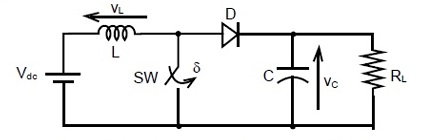
\includegraphics[width=0.5\columnwidth]{figs/Q 42.png}
    \caption{}
    \label{fig:placeholder}
\end{figure}
Under steady state operating conditions, the average voltage across the inductor and the capacitor respectively, are
\begin{multicols}{2}
    \begin{enumerate}
        \item $V_L = 0$ and $V_C = \frac{1}{1-\delta} V_{dc}$
        \item $V_L = \frac{\delta}{2} V_{dc}$ and $V_C = \frac{1}{1-\delta} V_{dc}$
        \item $V_L = 0$ and $V_C = \frac{\delta}{1-\delta} V_{dc}$
        \item $V_L = \frac{\delta}{2} V_{dc}$ and $V_C = \frac{\delta}{1-\delta} V_{dc}$
    \end{enumerate}
\end{multicols}
\item The single-phase full-bridge voltage source inverter (VSI), shown in figure, has an output frequency of 50 Hz. It uses unipolar pulse width modulation with switching frequency of 50 kHz and modulation index of 0.7. For $V_{in} = 100$ V DC, $L = 9.55$ mH, $C = 63.66\,\mu$F, and $R = 5\,\Omega$, the amplitude of the fundamental component in the output voltage $V_o$ (in Volt) under steady-state is \rule{3cm}{0.15mm}.\hfill{\textbf{(GATE EE 2015)}}
\begin{figure}[H]
    \centering
    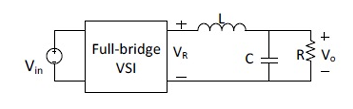
\includegraphics[width=0.5\columnwidth]{figs/Q 43.png}
    \caption{}
    \label{fig:placeholder}
\end{figure}
\item A 3-phase 50 Hz square wave (6-step) VSI feeds a 3-phase, 4 pole induction motor. The VSI line voltage has a dominant$ 5^{th}$ harmonic component. If the operating slip of the motor with respect to fundamental component voltage is 0.04, the slip of the motor with respect to $5^{th}$ harmonic component of voltage is \rule{2cm}{0.15mm}.\hfill{\textbf{(GATE EE 2015)}}

\item Consider a discrete time signal given by\hfill{\textbf{(GATE EE 2015)}}\\
$$
x[n] = (-0.25)^n\, u[n] + (0.5)^n\, u[-n-1]
$$
The region of convergence of its Z-transform would be
    \begin{enumerate}
        \item the region inside the circle of radius 0.5 and centered at origin
        \item the region outside the circle of radius 0.25 and centered at origin
        \item the annular region between the two circles, both centered at origin and having radii 0.25 and 0.5
        \item the entire Z plane
    \end{enumerate}

\item A parallel plate capacitor is partially filled with glass of dielectric constant 4.0 as shown below. The dielectric strengths of air and glass are 30 kV/cm and 300 kV/cm, respectively. The maximum voltage (in kilovolts), which can be applied across the capacitor without any breakdown, is \rule{3cm}{0.15mm}.\hfill{\textbf{(GATE EE 2015)}}
\begin{figure}[H]
    \centering
    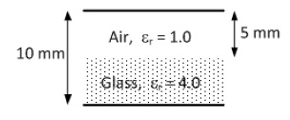
\includegraphics[width=0.5\columnwidth]{figs/Q 46.png}
    \caption{}
    \label{fig:placeholder}
\end{figure}

\item The figure shows a digital circuit constructed using negative edge triggered J-K flip flops. Assume a starting state of $Q_2Q_1Q_0=000$. This state $Q_2Q_1Q_0=000$ will repeat after \rule{3cm}{0.15mm} number of cycles of the clock CLK.\hfill{\textbf{(GATE EE 2015)}}
\begin{figure}[H]
    \centering
    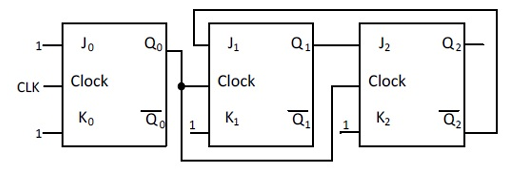
\includegraphics[width=0.5\columnwidth]{figs/Q 47.png}
    \caption{}
    \label{fig:placeholder}
\end{figure}
\item $f(A,B,C,D) = \prod M(0,1,3,4,5,7,9,11,12,13,14,15)$ is a maxterm representation of a Boolean function $f(A,B,C,D)$, where $A$ is the MSB and $D$ is the LSB. The equivalent minimized representation of this function is\hfill{\textbf{(GATE EE 2015)}}
    \begin{enumerate}
        \item $(A + C + D)(A + B + D)$
        \item $ACD + ABD$
        \item $ACD + ABCD + ABCD$
        \item $(B + C + D)(A + B + C + D)(A + B + C + D)$
    \end{enumerate}

\item The op-amp shown in the figure has a finite gain $A = 1000$ and an infinite input resistance. A step-voltage $V_1 = 1$ mV is applied at the input at time $t = 0$ as shown. Assuming that the operational amplifier is not saturated, the time constant (in millisecond) of the output voltage $V_o$ is\hfill{\textbf{(GATE EE 2015)}}
\begin{figure}[H]
    \centering
    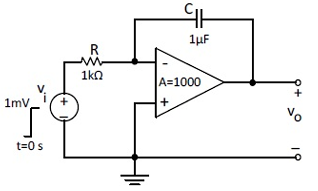
\includegraphics[width=0.5\columnwidth]{figs/Q 49.png}
    \caption{}
    \label{fig:placeholder}
\end{figure}
\begin{multicols}{4}
       \begin{enumerate}
        \item 1001
        \item 101
        \item 11
        \item 1
    \end{enumerate}
\end{multicols}

\item An 8-bit, unipolar Successive Approximation Register type ADC is used to convert 3.5 V to digital equivalent output. The reference voltage is +5 V. The output of the ADC, at the end of 3rd clock pulse after the start of conversion, is\hfill{\textbf{(GATE EE 2015)}}
\begin{multicols}{4}
    \begin{enumerate}
        \item 1010 0000
        \item 1000 0000
        \item 0000 0001
        \item 0000 0011
    \end{enumerate}
\end{multicols}
\item Consider the economic dispatch problem for a power plant having two generating units. The fuel costs in Rs/MWh along with the generation limits for the two units are given below:\hfill{\textbf{(GATE EE 2015)}}\\
$C_1(P_1) = 0.01P_1^2 + 30P_1 + 10;\ \ 100 \leq P_1 \leq 150$ MW\\
$C_2(P_2) = 0.05P_2^2 + 10P_2 + 10;\ \ 100 \leq P_2 \leq 180$ MW.\\
The incremental cost (in Rs/MWh) of the power plant when it supplies 200 MW is \rule{2cm}{0.15mm}.

\item Determine the correctness or otherwise of the following Assertion $[a]$ and the Reason $[r]$.\\
Assertion: Fast decoupled load flow method gives approximate load flow solution because it uses several assumptions.\\
Reason: Accuracy depends on the power mismatch vector tolerance.\hfill{\textbf{(GATE EE 2015)}}
    \begin{enumerate}
        \item Both $[a]$ and $[r]$ are true and $[r]$ is the correct reason for $[a]$.
        \item Both $[a]$ and $[r]$ are true but $[r]$ is not the correct reason for $[a]$.
        \item Both $[a]$ and $[r]$ are false.
        \item $[a]$ is false and $[r]$ is true.
    \end{enumerate}

\item A 50 Hz generating unit has $H$-constant of 2 MJ/MVA. The machine is initially operating in steady state at synchronous speed, and producing 1 pu of real power. The initial value of the rotor angle $\delta$ is $5^\circ$, when a bolted three phase to ground short circuit fault occurs at the terminal of the generator. Assuming the input mechanical power to remain at 1 pu, the value of $\delta$ in degrees, 0.02 second after the fault is \rule{3cm}{0.15mm}.\hfill{\textbf{(GATE EE 2015)}}

\item A sustained three-phase fault occurs in the power system shown in the figure. The current and voltage phasors during the fault (on a common reference), after the natural transients have died down, are also shown. Where is the fault located?\hfill{\textbf{(GATE EE 2015)}}
\begin{figure}[H]
    \centering
    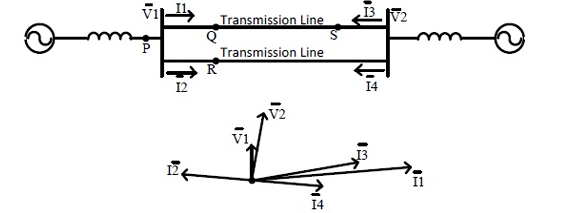
\includegraphics[width=0.7\columnwidth]{figs/Q 54.png}
    \caption{}
    \label{fig:placeholder}
\end{figure}
\begin{multicols}{4}
    \begin{enumerate}
        \item Location P
        \item Location Q
        \item Location R
        \item Location S
    \end{enumerate}
\end{multicols}
\item The circuit shown in the figure has two sources connected in series. The instantaneous voltage of the AC source (in Volt) is given by $v(t) = 12\sin t$. If the circuit is in steady state, then the rms value of the current (in Ampere) flowing in the circuit is \rule{3cm}{0.15mm}.\hfill{\textbf{(GATE EE 2015)}}
\begin{figure}[H]
    \centering
    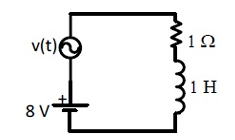
\includegraphics[width=0.5\columnwidth]{figs/Q 55.png}
    \caption{}
    \label{fig:placeholder}
\end{figure}
\item In a linear two-port network, when 10 V is applied to Port 1, a current of 4 A flows through Port 2 when it is short-circuited. When 5 V is applied to Port 1, a current of 1.25 A flows through a 1 $\Omega$ resistance connected across Port 2. When 3 V is applied to Port 1, the current (in Ampere) through a 2 $\Omega$ resistance connected across Port 2 is \rule{3cm}{0.15mm}.\hfill{\textbf{(GATE EE 2015)}}

\item In the given circuit, the parameter $k$ is positive, and the power dissipated in the $2\,\Omega$ resistor is 12.5 W. The value of $k$ is \rule{2cm}{0.15mm}.\hfill{\textbf{(GATE EE 2015)}}
\begin{figure}[H]
    \centering
    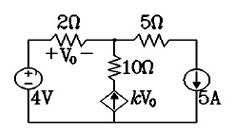
\includegraphics[width=0.5\columnwidth]{figs/Q 57.png}
    \caption{}
    \label{fig:placeholder}
\end{figure}
\item A separately excited DC motor runs at 1000 rpm on no load when its armature terminals are connected to a 200 V DC source and the rated voltage is applied to the field winding. The armature resistance of this motor is 1 $\Omega$. The no-load armature current is negligible. With the motor developing its full load torque, the armature voltage is set so that the rotor speed is 500 rpm. When the load torque is reduced to 50\% of the full load value under the same armature voltage conditions, the speed rises to 520 rpm. Neglecting the rotational losses, the full load armature current (in Ampere) is \rule{3cm}{0.15mm}.\hfill{\textbf{(GATE EE 2015)}}

\item A DC motor has the following specifications: 10 hp, 37.5 A, 230 V; flux/pole $=0.01$ Wb, number of poles $=4$, number of conductors $=666$, number of parallel paths $=2$. Armature resistance $=0.267~\Omega$. The armature reaction is negligible and rotational losses are 600 W. The motor operates from a 230 V DC supply. If the motor runs at 1000 rpm, the output torque produced (in Nm) is \rule{2cm}{0.15mm}.\hfill{\textbf{(GATE EE 2015)}}

\item A 200/400 V, 50 Hz, two-winding transformer is rated at 20 kVA. Its windings are connected as an auto-transformer of rating 200/600 V. A resistive load of 12 $\Omega$ is connected to the high voltage (600 V) side of the auto-transformer. The value of equivalent load resistance (in Ohm) as seen from low voltage side is\\ \rule{3cm}{0.15mm}.\hfill{\textbf{(GATE EE 2015)}}

\item Two single-phase transformers $T_1$ and $T_2$ each rated at 500 kVA are operated in parallel. Percentage impedances of $T_1$ and $T_2$ are $(1 + j6)$ and $(0.8 + j4.8)$, respectively. To share a load of 1000 kVA at 0.8 lagging power factor, the contribution of $T_2$ (in kVA) is \rule{3cm}{0.15mm}.\hfill{\textbf{(GATE EE 2015)}}

\item In the signal flow diagram given in the figure, $u_1$ and $u_2$ are possible inputs whereas $y_1$ and $y_2$ are possible outputs. When would the SISO system derived from this diagram be controllable and observable?\hfill{\textbf{(GATE EE 2015)}}
\begin{figure}[H]
    \centering
    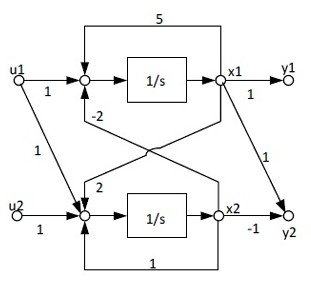
\includegraphics[width=0.5\columnwidth]{figs/Q 62.png}
    \caption{}
    \label{fig:placeholder}
\end{figure}
    \begin{enumerate}
        \item When $u_1$ is the only input and $y_1$ is the only output.
        \item When $u_2$ is the only input and $y_1$ is the only output.
        \item When $u_1$ is the only input and $y_2$ is the only output.
        \item When $u_2$ is the only input and $y_2$ is the only output.
    \end{enumerate}

\item The transfer function of a second order real system with a perfectly flat magnitude response of unity has a pole at $(2 - j3)$. List all the poles and zeroes.\hfill{\textbf{(GATE EE 2015)}}
    \begin{enumerate}
        \item Poles at $(2 \pm j3)$, no zeroes.
        \item Poles at $(\pm 2 - j3)$, one zero at origin.
        \item Poles at $(2 - j3)$, $(-2 + j3)$, zeroes at $(-2 - j3)$, $(2 + j3)$.
        \item Poles at $(2 \pm j3)$, zeroes at $(-2 \pm j3)$.
    \end{enumerate}

\item Find the transfer function $\dfrac{Y(s)}{X(s)}$ of the system given below.\hfill{\textbf{(GATE EE 2015)}}
\begin{figure}[H]
    \centering
    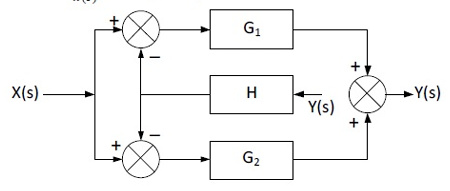
\includegraphics[width=0.5\columnwidth]{figs/Q 64.png}
    \caption{}
    \label{fig:placeholder}
\end{figure}
\begin{multicols}{2}
        \begin{enumerate}
        \item $\dfrac{G_1}{1-HG_1} + \dfrac{G_2}{1-HG_2}$
        \item $\dfrac{G_1}{1+HG_1} + \dfrac{G_2}{1+HG_2}$
        \item $\dfrac{G_1+G_2}{1+H(G_1+G_2)}$
        \item $\dfrac{G_1+G_2}{1-H(G_1+G_2)}$
    \end{enumerate}
\end{multicols}


\item The open loop poles of a third order unity feedback system are at $0, -1, -2$. Let the frequency corresponding to the point where the root locus of the system transits to unstable region be $K$. Now suppose we introduce a zero in the open loop transfer function at $-3$, while keeping all the earlier open loop poles intact. Which one of the following is TRUE about the point where the root locus of the modified system transits to unstable region?\hfill{\textbf{(GATE EE 2015)}}
    \begin{enumerate}
        \item It corresponds to a frequency greater than $K$
        \item It corresponds to a frequency less than $K$
        \item It corresponds to a frequency $K$
        \item Root locus of modified system never transits to unstable region
    \end{enumerate}
\end{enumerate}









\newpage
\begin{figure}[H]
    \centering
    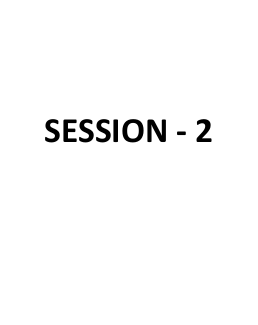
\includegraphics[width=1\columnwidth]{figs/image.png}
\end{figure}
\newpage
\begin{center}
\textbf{ Graduate Aptitude Test in Engineering}
  \end{center}
\textbf{Question Paper Name:}\quad EE:ELECTRICAL ENGINEERING 7th Feb Shift 1\\
\textbf{Number of Questions   :}\quad 65\\
\textbf{Total Marks:}\qquad \qquad \quad 100.0\\
\vspace{0.5cm}
Wrong answer for MCQ will result in negative marks, (-1/3) for 1 mark Questions and (-2/3) for 2 marks \\
\vspace{0.5cm}
General Aptitude \\
Number of Questions: 10\\
Section Marks: 15.0\\
\vspace{0.5cm}
 Q.1 to Q.5 carry 1 mark each \& Q.6 to Q.10 carry 2 marks each.\\
 \begin{enumerate}
 \item We \rule{3cm}{0.15mm} our friend's birthday and we \rule{3cm}{0.15mm} how to make it up to him.\hfill{\textbf{(GATE EE 2015)}}
    \begin{enumerate}
        \item completely forgot --- don’t just know
        \item forgot completely --- don’t just know
        \item completely forgot --- just don’t know
        \item forgot completely --- just don’t know
    \end{enumerate}

\item Choose the statement where underlined word is used correctly.\hfill{\textbf{(GATE EE 2015)}}

\begin{enumerate}
    \item The industrialist had a \underline{personnel} jet.
    \item I write my experience in my \underline{personnel} diary.
    \item All \underline{personnel} are being given the day off.
    \item Being religious is a \underline{personnel} aspect.
\end{enumerate}

\item A generic term that includes various items of clothing such as a skirt, a pair of trousers and a shirt is\hfill{\textbf{(GATE EE 2015)}}

\begin{multicols}{4}
\begin{enumerate}
    \item fabric
    \item textile
    \item fibre
    \item apparel
\end{enumerate}
\end{multicols}
\item Based on the given statements, select the most appropriate option to solve the given question.\hfill{\textbf{(GATE EE 2015)}}

What will be the total weight of 10 poles each of same weight?

\textbf{Statements:}

(I) One fourth of the weight of a pole is 5 kg.\\
(II) The total weight of these poles is 160 kg more than the total weight of two poles.


\begin{enumerate}
    \item Statement I alone is not sufficient.
    \item Statement II alone is not sufficient.
    \item Either I or II alone is sufficient.
    \item Both statements I and II together are not sufficient.
\end{enumerate}

\item Consider a function $f(x) = 1 - |x|$ on $-1 \leq x \leq 1$. The value of $x$ at which the function attains a maximum, and the maximum value of the function are:\hfill{\textbf{(GATE EE 2015)}}

\begin{multicols}{4}
\begin{enumerate}
    \item $0, -1$
    \item $-1, 0$
    \item $0, 1$
    \item $-1, 2$
\end{enumerate}
\end{multicols}

\item Out of the following four sentences, select the most suitable sentence with respect to grammar and usage:\hfill{\textbf{(GATE EE 2015)}}


\begin{enumerate}
    \item Since the report lacked needed information, it was of no use to them.
    \item The report was useless to them because there were no needed information in it.
    \item Since the report did not contain the needed information, it was not real useful to them.
    \item Since the report lacked needed information, it would not had been useful to them.
\end{enumerate}
\item In a triangle PQR, PS is the angle bisector of $\angle QPR$ and $\angle QPS = 60^\circ$. What is the length of PS?\hfill{\textbf{(GATE EE 2015)}}


\begin{multicols}{4}
\begin{enumerate}
    \item $\dfrac{(q+r)}{qr}$
    \item $\dfrac{qr}{(q+r)}$
    \item $\sqrt{(q^2 + r^2)}$
    \item $\dfrac{(q+r)^2}{qr}$
\end{enumerate}
\end{multicols}
\item If $p, q, r, s$ are distinct integers such that:\hfill{\textbf{(GATE EE 2015)}} \\
$f(p, q, r, s) = \max(p, q, r, s)$ \\
$g(p, q, r, s) = \min(p, q, r, s)$ \\
$h(p, q, r, s) =$ remainder of $(p \times q)/(r \times s)$ if $(p \times q) > (r \times s)$ or remainder of $(r \times s)/(p \times q)$ if $(r \times s) > (p \times q)$ \\

Also, a function $fgh(p, q, r, s) = f(p, q, r, s) \times g(p, q, r, s) \times h(p, q, r, s)$ \\
Also the same operations are valid with two variable functions of the form $f(p, q)$. \\

What is the value of $fg(h(2,5,7,3), 4, 6, 8)$?
\item If the list of letters, $P, R, S, T, U$ is an arithmetic sequence, which of the following are also in arithmetic sequence?\hfill{\textbf{(GATE EE 2015)}} \\

\begin{enumerate}
\item $2P, 2R, 2S, 2T, 2U$
\item $P-3, R-3, S-3, T-3, U-3$
\item $P^2, R^2, S^2, T^2, U^2$
\end{enumerate}

\begin{multicols}{4}
\begin{enumerate}
\item I only
\item I and II
\item II and III
\item I and III
\end{enumerate}
\end{multicols}
\item Four branches of a company are located at $M, N, O,$ and $P$. 
$M$ is north of $N$ at a distance of $4$ km; $P$ is south of $O$ at a distance of $2$ km; 
$N$ is southeast of $O$ by $1$ km. What is the distance between $M$ and $P$ in km?\hfill{\textbf{(GATE EE 2015)}} \\

\begin{multicols}{4}
\begin{enumerate}
\item (A) 5.34
\item (B) 6.74
\item (C) 28.5
\item (D) 45.49
\end{enumerate}
\end{multicols}
\newpage
\centering{ELECTRICAL ENGINNEERING}\\
Number of Questions:55\\
 Section Marks: 85\\
 \vspace{0.5cm
 }


\item Given $f(z) = g(z) + h(z)$, where $f, g, h$ are complex valued functions of a complex variable $z$. Which one of the following statements is TRUE? \hfill{\textbf{(GATE EE 2015)}}


\begin{enumerate}
\item  If $f(z)$ is differentiable at $z_0$, then $g(z)$ and $h(z)$ are also differentiable at $z_0$.
\item  If $g(z)$ and $h(z)$ are differentiable at $z_0$, then $f(z)$ is also differentiable at $z_0$.
\item  If $f(z)$ is continuous at $z_0$, then it is differentiable at $z_0$.
\item  If $f(z)$ is differentiable at $z_0$, then so are its real and imaginary parts.
\end{enumerate}

\item We have a set of $3$ linear equations in $3$ unknowns. 
`$X \equiv Y$' means $X$ and $Y$ are equivalent statements and 
`$X \not\equiv Y$' means $X$ and $Y$ are not equivalent statements. \\
P: There is a unique solution. \\
Q: The equations are linearly independent. \\
R: All eigenvalues of the coefficient matrix are nonzero. \\
S: The determinant of the coefficient matrix is nonzero. \\

Which one of the following is TRUE? \hfill{\textbf{(GATE EE 2015)}}

\begin{multicols}{2}
\begin{enumerate}
\item (A) $P \equiv Q \equiv R \equiv S$
\item (B) $P \equiv R \not\equiv Q \equiv S$
\item (C) $P \equiv Q \not\equiv R \equiv S$
\item (D) $P \not\equiv Q \not\equiv R \not\equiv S$
\end{enumerate}
\end{multicols}
\item Match the following. \hfill{\textbf{(GATE EE 2015)}}

\begin{figure}[H]
    \centering
    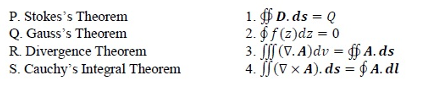
\includegraphics[width=0.8\columnwidth]{figs/2Q 13.png}

\end{figure}

\begin{multicols}{2}
\begin{enumerate}
\item P-2, Q-1, R-4, S-3
\item P-4, Q-1, R-3, S-2
\item P-4, Q-3, R-1, S-2
\item P-3, Q-4, R-2, S-1
\end{enumerate}
\end{multicols}

\item The Laplace transform of $f(t) = \dfrac{2\sqrt{t}}{\sqrt{\pi}}$ is $s^{-3/2}$. 
The Laplace transform of $g(t) = \dfrac{1}{\sqrt{\pi t}}$ is \\\hfill{\textbf{(GATE EE 2015)}}

\begin{multicols}{4}
\begin{enumerate}
\item $ \dfrac{3}{2} s^{-5/2} $
\item $ s^{-1/2} $
\item $ s^{1/2} $
\item $ s^{3/2} $
\end{enumerate}
\end{multicols}
\item Match the following. \hfill{\textbf{(GATE EE 2015)}}
\begin{figure}[H]
    \centering
    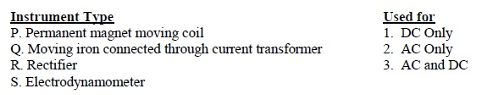
\includegraphics[width=0.8\columnwidth]{figs/2Q 15.png}
\end{figure}

\begin{multicols}{2}
\begin{enumerate}
\item P-1, Q-2, R-1, S-3
\item P-1, Q-3, R-1, S-2
\item P-1, Q-2, R-3, S-3
\item P-3, Q-1, R-2, S-1
\end{enumerate}
\end{multicols}
\item A 3-phase balanced load which has a power factor of $0.707$ is connected to a balanced supply. 
The power consumed by the load is $5 \, \text{kW}$. 
The power is measured by the two-wattmeter method. 
The readings of the two wattmeters are\hfill{\textbf{(GATE EE 2015)}}

\begin{multicols}{2}
\begin{enumerate}
\item 3.94 kW and 1.06 kW
\item 2.50 kW and 2.50 kW
\item 5.00 kW and 0.00 kW
\item 2.96 kW and 2.04 kW
\end{enumerate}
\end{multicols}
\item A capacitive voltage divider is used to measure the bus voltage $V_{bus}$ in a high-voltage 50 Hz AC system as shown in the figure. 
The measurement capacitors $C_1$ and $C_2$ have tolerances of $\pm 10\%$ on their nominal capacitance values. 
If the bus voltage $V_{bus}$ is $100 \, \text{kV rms}$, the maximum rms output voltage $V_{out}$ (in kV), considering the capacitor tolerances, is\rule{3cm}{0.15mm}.\hfill{\textbf{(GATE EE 2015)}}
\begin{figure}[H]
    \centering
    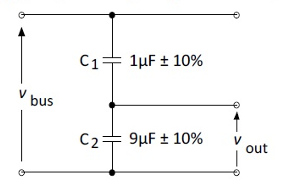
\includegraphics[width=0.5\columnwidth]{figs/2Q 17.png}
    \caption{}
    \label{fig:placeholder}
\end{figure}

\item In the following circuit, the input voltage $V_{in}$ is $100 \sin(100 \pi t)$. 
For $100 \pi R C = 50$, the average voltage across $R$ (in Volts) under steady-state is nearest\hfill{\textbf{(GATE EE 2015)}}
\begin{figure}[H]
    \centering
    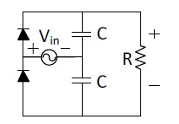
\includegraphics[width=0.5\columnwidth]{figs/2Q 18.png}
    \caption{}
    \label{fig:placeholder}
\end{figure}
\begin{multicols}{4}
\begin{enumerate}
\item 100
\item 31.8
\item 200
\item 63.6
\end{enumerate}
\end{multicols}

\item Two semi-infinite dielectric regions are separated by a plane boundary at $y = 0$. 
The dielectric constants of region 1 ($y < 0$) and region 2 ($y > 0$) are $2$ and $5$, respectively. 
Region 1 has uniform electric field 
\begin{align}
\vec{E} = 3\hat{a}_x + 4\hat{a}_y + 2\hat{a}_z,
\end{align}
where $\hat{a}_x, \hat{a}_y, \hat{a}_z$ are unit vectors along the $x, y, z$ axes, respectively. 
The electric field in region 2 is\hfill{\textbf{(GATE EE 2015)}}

\begin{multicols}{2}
\begin{enumerate}
\item $3\hat{a}_x + 1.6\hat{a}_y + 2\hat{a}_z$
\item $1.2\hat{a}_x + 4\hat{a}_y + 2\hat{a}_z$
\item $1.2\hat{a}_x + 4\hat{a}_y + 0.8\hat{a}_z$
\item $3\hat{a}_x + 10\hat{a}_y + 0.8\hat{a}_z$
\end{enumerate}
\end{multicols}

\item A circular turn of radius $1 \, \text{m}$ revolves at $60 \, \text{rpm}$ about its diameter aligned with the x-axis as shown in the figure. 
The value of $\mu_0$ is $4\pi \times 10^{-7}$ in SI unit. If a uniform magnetic field intensity \hfill{\textbf{(GATE EE 2015)}}
\begin{align}
\vec{H} = 10^7 \hat{z} \, \text{A/m}
\end{align}
is applied, then the peak value of the induced voltage, $V_{turn}$ (in Volts), is
\begin{figure}[H]
    \centering
    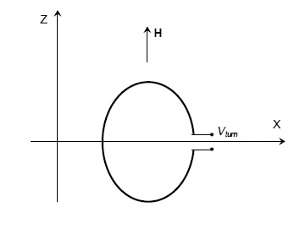
\includegraphics[width=0.5\columnwidth]{figs/2Q 20.png}
    \caption{}
    \label{fig:placeholder}
\end{figure}

\item The operational amplifier shown in the figure is ideal. The input voltage (in Volt) is
\begin{align}
V_{i} = 2\sin(2\pi \times 2000t)
\end{align}
The amplitude of the output voltage $V_o$ (in Volt) is $\underline{\hspace{2cm}}$\hfill{\textbf{(GATE EE 2015)}}
\begin{figure}[H]
    \centering
    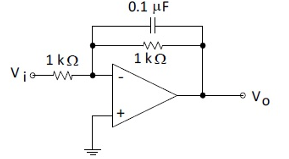
\includegraphics[width=0.5\columnwidth]{figs/2Q 21.png}
    \caption{}
    \label{fig:placeholder}
\end{figure}
\item In the following circuit, the transistor is in active mode and $V_C = 2\,\text{V}$. To get $V_C = 4\,\text{V}$, we replace $R_C$ with $R_C'$. Then the ratio $R_C'/R_C$ is $\underline{\hspace{2cm}}$\hfill{\textbf{(GATE EE 2015)}}
\begin{figure}[H]
    \centering
    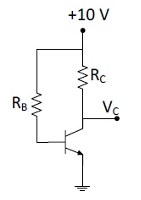
\includegraphics[width=0.3\columnwidth]{figs/2Q 22.png}
    \caption{}
    \label{fig:placeholder}
\end{figure}
\item Consider the following Sum of Products expression, $F$.
\begin{align}
F = ABC + \overline{A}BC + AB\overline{C} + \overline{A}B\overline{C}
\end{align}
The equivalent Product of Sums expression is\hfill{\textbf{(GATE EE 2015)}}


\begin{enumerate}
    \item $(A + \overline{B} + C)(\overline{A} + B + C)(\overline{A} + B + \overline{C})$
    \item $(A + B + \overline{C})(A + \overline{B} + C)(\overline{A} + B + C)$
    \item $(A + B + \overline{C})(A + \overline{B} + C)(A + B + C)$
    \item $(\overline{A} + \overline{B} + C)(A + B + \overline{C})(A + B + C)$
\end{enumerate}

\item The filters F1 and F2 having characteristics as shown in Figures (a) and (b) are connected as shown in Figure (c). 
\begin{figure}[H]
    \centering
    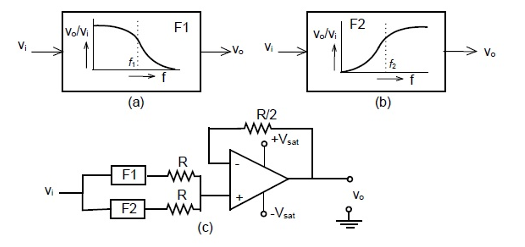
\includegraphics[width=0.75\columnwidth]{figs/2Q 24.png}
    \caption{}
    \label{fig:placeholder}
\end{figure}
The cut-off frequencies of F1 and F2 are $f_1$ and $f_2$ respectively. If $f_1 < f_2$, the resultant circuit exhibits the characteristic of a\hfill{\textbf{(GATE EE 2015)}}
\begin{multicols}{2}
\begin{enumerate}
    \item Band-pass filter
    \item Band-stop filter
    \item All pass filter
    \item High-Q filter
\end{enumerate}
\end{multicols}

\item When a bipolar junction transistor is operating in the saturation mode, which one of the following statements is TRUE about the state of its collector-base (CB) and the base-emitter (BE) junctions?\hfill{\textbf{(GATE EE 2015)}}

\begin{enumerate}
    \item The CB junction is forward biased and the BE junction is reverse biased.
    \item The CB junction is reverse biased and the BE junction is forward biased.
    \item Both the CB and BE junctions are forward biased.
    \item Both the CB and BE junctions are reverse biased.
\end{enumerate}

\item The synchronous generator shown in the figure is supplying active power to an infinite bus via two short, lossless transmission lines, and is initially in steady state. The mechanical power input to the generator and the voltage magnitude $E$ are constant. If one line is tripped at time $t_1$ by opening the circuit breakers at the two ends (although there is no fault), then it is seen that the generator undergoes a stable transient. Which one of the following waveforms of the rotor angle $\delta$ shows the transient correctly?\\\hfill{\textbf{(GATE EE 2015)}}
\begin{figure}[H]
    \centering
    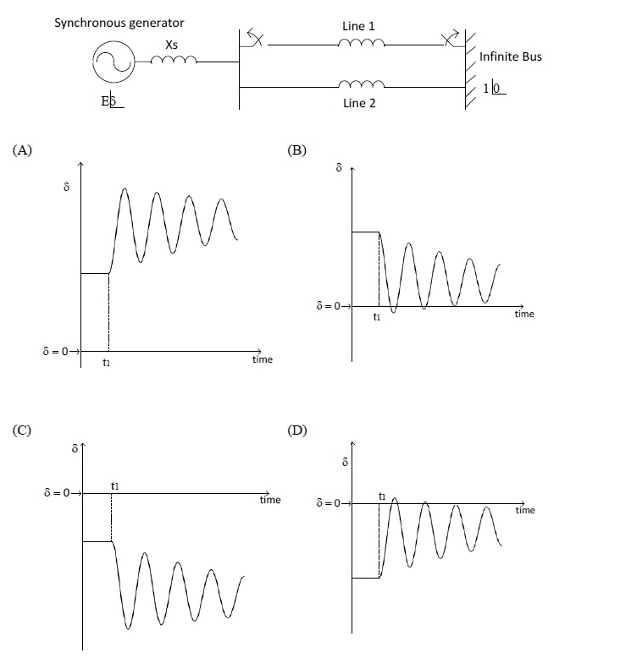
\includegraphics[width=1\columnwidth]{figs/2Q 26.png}
    \caption{}
    \label{fig:placeholder}
\end{figure}


\item A 3-bus power system network consists of 3 transmission lines. The bus admittance matrix of the uncompensated system is\\
\myvec{

-j6 & j3 & j4 \\
j3 & -j7 & j5 \\
j4 & j5 & -j8
}pu.\\
If the shunt capacitance of all transmission lines is 50\% compensated, the imaginary part of the $3^{\text{rd}}$ row $3^{\text{rd}}$ column element (in pu) of the bus admittance matrix after compensation is\hfill{\textbf{(GATE EE 2015)}}

\begin{multicols}{4}
\begin{enumerate}
    \item $-j7.0$
    \item $-j8.5$
    \item $-j7.5$
    \item $-j9.0$
\end{enumerate}
\end{multicols}

\vspace{0.5cm}

\item A series RL circuit is excited at $t = 0$ by closing a switch as shown in the figure. Assuming zero initial conditions, the value of $\dfrac{d^2i}{dt^2}$ at $t=0^+$ is\hfill{\textbf{(GATE EE 2015)}}
\begin{figure}[H]
    \centering
    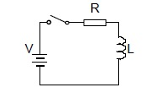
\includegraphics[width=0.5\columnwidth]{figs/2Q 28.png}
    \caption{}
    \label{fig:placeholder}
\end{figure}

\begin{multicols}{4}
\begin{enumerate}
    \item $\dfrac{V}{L}$
    \item $-\dfrac{V}{R}$
    \item $0$
    \item $-\dfrac{RV}{L^2}$
\end{enumerate}
\end{multicols}


\item The current $i$ (in Ampere) in the $2~\Omega$ resistor of the given network  is $\underline{\hspace{2cm}}$ \hfill{\textbf{(GATE EE 2015)}}
\begin{figure}[H]
    \centering
    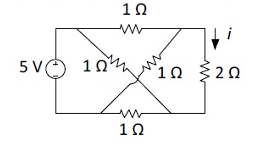
\includegraphics[width=0.5\columnwidth]{figs/2Q 29.png}
    \caption{}
    \label{fig:placeholder}
\end{figure}

\item Find the transformer ratios $a$ and $b$ such that the impedance ($Z_\text{in}$) is resistive and equals $2.5~\Omega$ when the network is excited with a sine wave voltage of angular frequency of $5000$~rad/s.\hfill{\textbf{(GATE EE 2015)}}
\begin{figure}[H]
    \centering
    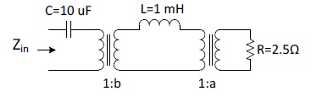
\includegraphics[width=0.7\columnwidth]{figs/2Q 30.png}
    \caption{}
    \label{fig:placeholder}
\end{figure}

\begin{multicols}{2}
\begin{enumerate}
    \item $a = 0.5,\quad b = 2.0$
    \item $a = 2.0,\quad b = 0.5$
    \item $a = 1.0,\quad b = 1.0$
    \item $a = 4.0,\quad b = 0.5$
\end{enumerate}
\end{multicols}

\vspace{0.5cm}

\item A shunt-connected DC motor operates at its rated terminal voltage. Its no-load speed is $200$ radian/second. At its rated torque of $500$ Nm, its speed is $180$ radian/second. The motor is used to directly drive a load whose load torque $T_L$ depends on its rotational speed $\omega_r$ (in radian/second), such that $T_L = 2.78 \times \omega_r$. Neglecting rotational losses, the steady-state speed (in radian/second) of the motor, when it drives this load, is $\underline{\hspace{2cm}}$\hfill{\textbf{(GATE EE 2015)}}


\item The figure shows the per-phase equivalent circuit of a two-pole three-phase induction motor operating at $50$ Hz. The "air-gap" voltage, $V_g$ across the magnetizing inductance, is $210$ V rms, and the slip, $s$, is $0.05$. The torque (in Nm) produced by the motor is $\underline{\hspace{2cm}}$\hfill{\textbf{(GATE EE 2015)}}
\begin{figure}[H]
    \centering
    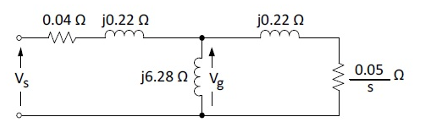
\includegraphics[width=0.75\columnwidth]{figs/2Q 32.png}
    \caption{}
    \label{fig:placeholder}
\end{figure}

\item A 4-pole, separately excited, wave wound DC machine with negligible armature resistance is rated for $230$~V and $5$~kW at a speed of $1200$~rpm. If the same armature coils are reconnected to form a lap winding, what is the rated voltage (in volts) and power (in kW) respectively at $1200$~rpm of the reconnected machine if the field circuit is left unchanged?\hfill{\textbf{(GATE EE 2015)}}

\begin{multicols}{4}
\begin{enumerate}
    \item $230$ and $5$
    \item $115$ and $5$
    \item $115$ and $2.5$
    \item $230$ and $2.5$
\end{enumerate}
\end{multicols}

\item An open loop control system results in a response of $e^{-2t}(\sin 5t + \cos 5t)$ for a unit impulse input. The DC gain of the control system is $\underline{\hspace{2cm}}$\hfill{\textbf{(GATE EE 2015)}}
\item Nyquist plots of two functions $G_1(s)$ and $G_2(s)$ are shown in figure.
\begin{figure}[H]
    \centering
    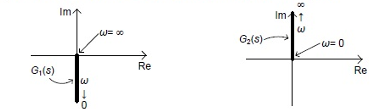
\includegraphics[width=0.5\columnwidth]{figs/2Q 35.png}
    \caption{}
    \label{fig:placeholder}
\end{figure}


Nyquist plot of the product of $G_1(s)$ and $G_2(s)$ is\hfill{\textbf{(GATE EE 2015)}}
\begin{figure}
    \centering
    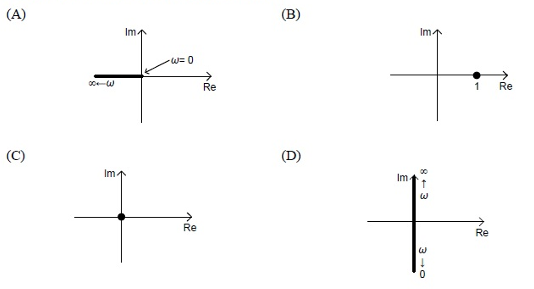
\includegraphics[width=0.9\columnwidth]{figs/2Q 35 opt.png}
\end{figure}

\item The volume enclosed by the surface $f(x,y) = e^x$ over the triangle bounded by the lines $x = y$, $x = 0$, $y = 1$ in the $xy$ plane is $\underline{\hspace{2cm}}$\hfill{\textbf{(GATE EE 2015)}}


\item Two coins R and S are tossed. The 4 joint events $H_RH_S$, $T_RT_S$, $H_RT_S$, $T_RH_S$ have probabilities $0.28, 0.18, 0.30, 0.24$ respectively, where $H$ represents head and $T$ represents tail. Which one of the following is TRUE?\hfill{\textbf{(GATE EE 2015)}}

\begin{enumerate}
    \item The coin tosses are independent.
    \item R is fair, S is not.
    \item S is fair, R is not.
    \item The coin tosses are dependent.
\end{enumerate}

\item A differential equation $\frac{di}{dt} - 0.2i = 0$ is applicable over $-10 < t < 10$. If $i(4) = 10$, then $i(-5)$ is $\underline{\hspace{2cm}}$\hfill{\textbf{(GATE EE 2015)}}
\item Consider a signal defined by\hfill{\textbf{(GATE EE 2015)}}
\begin{align}
x(t) = 
\begin{cases}
e^{j10t} & \text{for } |t| \leq 1 \\
0 & \text{for } |t| > 1
\end{cases}
\end{align}
Its Fourier Transform is

\begin{multicols}{2}
\begin{enumerate}
    \item $\dfrac{2 \sin (\omega - 10)}{\omega - 10}$
    \item $2 e^{j10} \dfrac{\sin (\omega - 10)}{\omega - 10}$
    \item $\dfrac{2 \sin \omega}{\omega - 10}$
    \item $e^{j10\omega} \dfrac{2 \sin \omega}{\omega}$
\end{enumerate}
\end{multicols}

\vspace{0.5cm}

\item The coils of a wattmeter have resistances $0.01~\Omega$ and $1000~\Omega$; their inductances may be neglected. The wattmeter is connected as shown in the figure, to measure the power consumed by a load, which draws $25$~A at power factor $0.8$. The voltage across the load terminals is $30$~V. The percentage error on the wattmeter reading is $\underline{\hspace{2cm}}$\hfill{\textbf{(GATE EE 2015)}}
\begin{figure}[H]
    \centering
    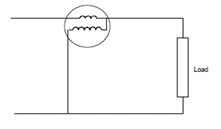
\includegraphics[width=0.5\columnwidth]{figs/2Q 40.png}
    \caption{}
    \label{fig:placeholder}
\end{figure}

\item A buck converter feeding a variable resistive load is shown in the figure. The switching frequency of the switch S is 100 kHz and the duty ratio is 0.6. The output voltage $V_o$ is 36 V. Assume that all the components are ideal, and that the output voltage is ripple-free. The value of $R$ (in Ohm) that will make the inductor current $(i_L)$ just continuous is \rule{2cm}{0.15mm}.\hfill{\textbf{(GATE EE 2015)}}
\begin{figure}[H]
    \centering
    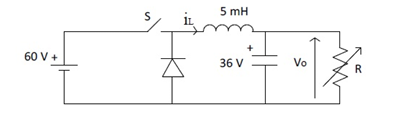
\includegraphics[width=0.8\columnwidth]{figs/2Q 41.png}
    \caption{}
    \label{fig:placeholder}
\end{figure}

\item For the switching converter shown in the following figure, assume steady-state operation. Also assume that the components are ideal, the inductor current is always positive and continuous and switching period is $T_s$. If the voltage $V_L$ is as shown, the duty cycle of the switch S is \rule{2cm}{0.15mm}.\hfill{\textbf{(GATE EE 2015)}}
\begin{figure}[H]
    \centering
    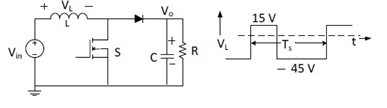
\includegraphics[width=0.75\columnwidth]{figs/2Q 42.png}
    \caption{}
    \label{fig:placeholder}
\end{figure}

\item In the given rectifier, the delay angle of the thyristor $T_1$ measured from the positive going zero crossing of $V_s$ is $30^\circ$. If the input voltage $V_s$ is $100\sin(100\pi t)$ V, the average voltage across $R$ (in Volt) under steady-state is \rule{2cm}{0.15mm}.\hfill{\textbf{(GATE EE 2015)}}
\begin{figure}[H]
    \centering
    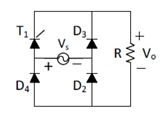
\includegraphics[width=0.5\columnwidth]{figs/2Q 43.png}
    \caption{}
    \label{fig:placeholder}
\end{figure}

\item For linear time invariant systems, that are Bounded Input Bounded Output stable, which one of the following statements is TRUE?\hfill{\textbf{(GATE EE 2015)}}
    \begin{enumerate}
        \item The impulse response will be integrable, but may not be absolutely integrable.
        \item The unit impulse response will have finite support.
        \item The unit step response will be absolutely integrable.
        \item The unit step response will be bounded.
    \end{enumerate}

\item The z-Transform of a sequence $x[n]$ is given as $X(z) = 2z + 4 - 4/z + 3/z^2$. If $y[n]$ is the first difference of $x[n]$, then $Y(z)$ is given by\hfill{\textbf{(GATE EE 2015)}}
    \begin{enumerate}
        \item $2z + 2 - 8/z + 7/z^2 - 3/z^3$
        \item $2z - 2 - 6/z + 1/z^2 - 3/z^3$
        \item $-2z - 2 + 8/z - 7/z^2 + 3/z^3$
        \item $4z - 2 - 8/z - 1/z^2 + 3/z^3$
    \end{enumerate}

\item Two semi-infinite conducting sheets are placed at right angles to each other as shown in the figure. A point charge of $+Q$ is placed at a distance of $d$ from both sheets. The net force on the charge is
$ \frac{Q^2}{4\pi \epsilon_0 d^2} K $
where $K$ is given by\hfill{\textbf{(GATE EE 2015)}}
\begin{figure}[H]
    \centering
    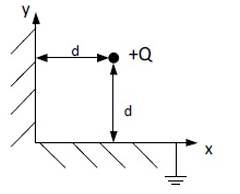
\includegraphics[width=0.4\columnwidth]{figs/2Q 46.png}
    \caption{}
    \label{fig:placeholder}
\end{figure}

  \begin{multicols}{4}
    \begin{enumerate}
        \item $0$
        \item $\frac{1}{4} i - \frac{1}{4} j$
        \item $-\frac{1}{8} i - \frac{1}{8} j$
        \item $\frac{1 - 2\sqrt{2}}{8\sqrt{2}} i + \frac{1 - 2\sqrt{2}}{8\sqrt{2}} j$
    \end{enumerate}
\end{multicols}
\item In the following sequential circuit, the initial state (before the first clock pulse) of the circuit is $Q_1Q_0 = 00$. The state $(Q_1 Q_0)$, immediately after the $333^{\text{rd}}$ clock pulse is\\\hfill{\textbf{(GATE EE 2015)}}
\begin{figure}[H]
    \centering
    \includegraphics[width=0.6\columnwidth]{figs/2Q 47.png}
    \caption{}
    \label{fig:placeholder}
\end{figure}

\begin{multicols}{4}
    \begin{enumerate}
        \item 00
        \item 01
        \item 10
        \item 11
    \end{enumerate}
\end{multicols}
\item A Boolean function $f(A,B,C,D) = \prod(1,5,12,15)$ is to be implemented using an $8 \times 1$ multiplexer (A is MSB). The inputs $ABC$ are connected to the select inputs $S_2, S_1, S_0$ of the multiplexer respectively.
\begin{figure}[H]
    \centering
    \includegraphics[width=0.5\columnwidth]{figs/2Q 48.png}
    \caption{}
    \label{fig:placeholder}
\end{figure}
Which one of the following options gives the correct inputs to pins 0,1,2,3,4,5,6,7 in order? \hfill{\textbf{(GATE EE 2015)}}
    \begin{enumerate}
        \item $D, 0, D, 0, 0, 0, D, D$
        \item $D, 1, D, 1, 1, 1, D, D$
        \item $D, 1, D, 1, 1, 1, D, D$
        \item $D, 0, D, 0, 0, 0, D, D$
    \end{enumerate}

\item The saturation voltage of the ideal op-amp shown below is $\pm 10$ V. The output voltage $v_o$ of the following circuit in the steady-state is\hfill{\textbf{(GATE EE 2015)}}
\begin{figure}[H]
    \centering
    \includegraphics[width=0.5\columnwidth]{figs/2Q 49.png}
    \caption{}
    \label{fig:placeholder}
\end{figure}
\begin{multicols}{2}
    \begin{enumerate}
        \item square wave of period 0.55 ms
        \item triangular wave of period 0.55 ms
        \item square wave of period 0.25 ms
        \item triangular wave of period 0.25 ms
    \end{enumerate}
\end{multicols}
\item The incremental costs (in Rupees/MWh) of operating two generating units are functions of their respective powers $P_1$ and $P_2$ in MW, and are given by\\
$\frac{dC_1}{dP_1}=0.2P_1+50$\\
$\frac{dC_2}{dP_2}=0.24P_2+40$\\
where\\ $20MW \leq P_1 \leq 150$ MW, $20MW \leq P_2 \leq 150$ MW.\\
For a certain load demand, $P_1$ and $P_2$ have been chosen such that $\frac{dC_1}{dP_1}=76$ Rs/MWh and $\frac{dC_2}{dP_2}=68.8$ Rs/MWh. If the generations are rescheduled to minimize the total cost, then $P_2$ is \rule{2cm}{0.15mm}.\hfill{\textbf{(GATE EE 2015)}}

\item A composite conductor consists of three conductors of radius $R$ each. The conductors are arranged as shown below. The geometric mean radius (GMR) (in cm) of the composite conductor is $kR$. The value of $k$ is \rule{3cm}{0.15mm}.\hfill{\textbf{(GATE EE 2015)}}
\begin{figure}[H]
    \centering
    \includegraphics[width=0.4\columnwidth]{figs/2Q 51.png}
    \caption{}
    \label{fig:placeholder}
\end{figure}
\item A 3-phase transformer rated for 33 kV/11 kV is connected in delta/star as shown in figure. The current transformers (CTs) on low and high voltage sides have a ratio of 500/5. Find the currents $i_1$ and $i_2$, if the fault current is 300 A as shown in figure.\\\hfill{\textbf{(GATE EE 2015)}}
\begin{figure}[H]
    \centering
    \includegraphics[width=0.8\columnwidth]{figs/2Q 52.png}
    \caption{}
    \label{fig:placeholder}
\end{figure}
\begin{multicols}{2}
     \begin{enumerate}
        \item $i_1 = 1/\sqrt{3}$ A, $i_2 = 0$ A
        \item $i_1 = 0$, $i_2 = 0$ A
        \item $i_1 = 0$, $i_2 = 1/\sqrt{3}$ A
        \item $i_1 = 1/\sqrt{3}$ A, $i_2 = 1/\sqrt{3}$ A
    \end{enumerate}
\end{multicols}
   

\item A balanced (positive sequence) three-phase AC voltage source is connected to a balanced, star connected load through a star-delta transformer as shown in the figure. The line-to-line voltage rating is 230 V on the star side, and 115 V on the delta side. If the magnetizing current is neglected and $I_s = 100 \angle 0^\circ$ A, then what is the value of $I_p$ in Ampere?\hfill{\textbf{(GATE EE 2015)}}
\begin{figure}[H]
    \centering
    \includegraphics[width=0.8\columnwidth]{figs/2Q 53.png}
    \caption{}
    \label{fig:placeholder}
\end{figure}
\begin{multicols}{4}
    \begin{enumerate}
        \item $50 \angle 230^\circ$
        \item $50 \angle -30^\circ$
        \item $50\sqrt{3}\angle 230^\circ$
        \item $200\angle 230^\circ$
    \end{enumerate}
\end{multicols}
\item In the given network $V_1 = 100\angle 0^\circ$ V, $V_2 = 100\angle -120^\circ$ V, $V_3 = 100\angle +120^\circ$ V. The phasor current $i$ (in Ampere) is\hfill{\textbf{(GATE EE 2015)}}
\begin{figure}[H]
    \centering
    \includegraphics[width=0.5\columnwidth]{figs/2Q 54.png}
    \caption{}
    \label{fig:placeholder}
\end{figure}
\begin{multicols}{4}
    \begin{enumerate}
        \item $173.2\angle -60^\circ$
        \item $173.2\angle 120^\circ$
        \item $100.0\angle -60^\circ$
        \item $100.0\angle 120^\circ$
    \end{enumerate}
\end{multicols}

\item A symmetrical square wave of 50\% duty cycle has amplitude of $\pm 15$ V and time period of $0.4\pi$ ms. This square wave is applied across a series RLC circuit with $R = 5~\Omega$, $L = 10$ mH, and $C = 4~\mu$F. The amplitude of the 5000 rad/s component of the capacitor voltage (in Volt) is \rule{3cm}{0.15mm}.\hfill{\textbf{(GATE EE 2015)}}
\begin{figure}[H]
    \centering
    \includegraphics[width=0.5\columnwidth]{figs/2Q 55.png}
    \caption{}
    \label{fig:placeholder}
\end{figure}

\item Two identical coils each having inductance $L$ are placed together on the same core. If an overall inductance of $\alpha L$ is obtained by interconnecting these two coils, the minimum value of $\alpha$ is \rule{3cm}{0.15mm}.\hfill{\textbf{(GATE EE 2015)}}

\item A three-winding transformer is connected to an AC voltage source as shown in the figure. The number of turns are as follows: $N_1 = 100$, $N_2 = 50$, $N_3 = 50$. If the magnetizing current is neglected, and the currents in two windings are $I_2 = 2\angle30^\circ$ A and $I_3 = 2\angle150^\circ$ A, then what is the value of the current $I_1$ in Ampere?\hfill{\textbf{(GATE EE 2015)}}
\begin{figure}[H]
    \centering
    \includegraphics[width=0.5\columnwidth]{figs/2Q 57.png}
    \caption{}
    \label{fig:placeholder}
\end{figure}
\begin{multicols}{4}
    \begin{enumerate}
        \item $1\angle 290^\circ$
        \item $1\angle 270^\circ$
        \item $4\angle 290^\circ$
        \item $4\angle 270^\circ$
    \end{enumerate}
\end{multicols}
\item With an armature voltage of 100 V and rated field winding voltage, the speed of a separately excited DC motor driving a fan is 1000 rpm, and its armature current is 10 A. The armature resistance is $1~\Omega$. The load torque of the fan load is proportional to the square of the rotor speed. Neglecting rotational losses, the value of the armature voltage (in Volt) which will reduce the rotor speed to 500 rpm is \rule{3cm}{0.15mm}.\hfill{\textbf{(GATE EE 2015)}}

\item A three-phase, 11 kV, 50 Hz, 2 pole, star connected, cylindrical rotor synchronous motor is connected to an 11 kV, 50 Hz source. Its synchronous reactance is $50~\Omega$ per phase, and its stator resistance is negligible. The motor has a constant field excitation. At a particular load torque, its stator current is 100 A at unity power factor. If the load torque is increased so that the stator current is 120 A, then the load angle (in degrees) at this load is \rule{3cm}{0.15mm}.\hfill{\textbf{(GATE EE 2015)}}

\item A 220 V, 3-phase, 4-pole, 50 Hz inductor motor of wound rotor type is supplied at rated voltage and frequency. The stator resistance, magnetizing reactance, and core loss are negligible. The maximum torque produced by the rotor is 225\% of full load torque and it occurs at 15\% slip. The actual rotor resistance is $0.03~\Omega$/phase. The value of external resistance (in Ohm) which must be inserted in a rotor phase if the maximum torque is to occur at start is \rule{3cm}{0.15mm}.\hfill{\textbf{(GATE EE 2015)}}

\item Two three-phase transformers are realized using single-phase transformers as shown in the figure.\hfill{\textbf{(GATE EE 2015)}}
\begin{figure}[H]
    \centering
    \includegraphics[width=0.75\columnwidth]{figs/2Q 61.png}
    \caption{}
    \label{fig:placeholder}
\end{figure}
 The phase difference (in degree) between voltages $V_1$ and $V_2$ is \rule{3cm}{0.15mm}.
\item The following discrete-time equations result from the numerical integration of the differential equations of an un-damped simple harmonic oscillator with state variables $x$ and $y$. The integration time step is $h$.\hfill{\textbf{(GATE EE 2015)}}
\begin{align}
  \frac{x_{k+1} - x_k}{h} = y_k\\
\frac{y_{k+1} - y_k}{h} = -x_k
\end{align}

For this discrete-time system, which one of the following statements is TRUE?
    \begin{enumerate}
        \item The system is not stable for $h > 0$
        \item The system is stable for $h > \frac{1}{2}$
        \item The system is stable for $0 < h < \frac{1}{\pi}$
        \item The system is stable for $\frac{1}{2\pi} < h < \frac{1}{2}$
    \end{enumerate}
\item The unit step response of a system with the transfer function $G(s) = \frac{1 - 2s}{1 + s}$ is given by which one of the following waveforms?\hfill{\textbf{(GATE EE 2015)}}
  \begin{figure}[H]
      \centering
      \includegraphics[width=1\columnwidth]{figs/2Q 63.png}
      \caption{}
      \label{fig:placeholder}
  \end{figure}

\item An open loop transfer function $G(s)$ of a system is\hfill{\textbf{(GATE EE 2015)}}
$$
G(s) = \frac{K}{s(s+1)(s+2)}
$$\\
For a unity feedback system, the breakaway point of the root loci on the real axis occurs at,
\begin{multicols}{2}
        \begin{enumerate}
        \item $-0.42$
        \item $-1.58$
        \item $-0.42$ and $-1.58$
        \item none of the above
    \end{enumerate}
\end{multicols}


\item For the system governed by the set of equations:\hfill{\textbf{(GATE EE 2015)}}\\
$dx_1/dt = 2x_1 + x_2 + u$\\
$dx_2/dt = -2x_1 + u$\\
$y = 3x_1$\\
the transfer function $Y(s)/U(s)$ is given by
\begin{multicols}{2}
    \begin{enumerate}
        \item $\frac{3(s+1)}{(s^2 - 2s + 2)}$
        \item $\frac{3(2s+1)}{(s^2 - 2s + 1)}$
        \item $\frac{(s+1)}{(s^2 - 2s + 1)}$
        \item $\frac{3(2s+1)}{(s^2 - 2s + 2)}$
    \end{enumerate}
\end{multicols}


 \end{enumerate}
\end{document}



